\section{Інтерпретація результатів моделювання, формулювання висновків та пропозицій}

\subsection{Інтерпретація результатів моделювання}

Верифікована модель (розділ~3) відтворює правила системи за припущення $M = 2$ і в окремих
випадках збігається з аналітичним розвʼязком; фактори -- названі метою моделювання стратегія й
інтенсивність надходження. За потоку з умови памʼяті бракує 17,5~\% і черга зростає необмежено
(рисунок~\ref{fig:exp-unstable}), тому інтенсивності зменшено коефіцієнтом~$\gamma$, а для
заданого потоку потрібна зміна ресурсу. Уже за $\gamma = 0{,}8$ стійкість втрачають стратегії 1--2: поки завдання~C чекає обох
одиниць памʼяті, вивільнена одиниця простоює.

Вплив стратегії зростає з навантаженням: за $\gamma = 0{,}4$ середній час перебування в різних
стратегіях відрізняється на чверть, а за $\gamma = 0{,}7$ -- більш ніж удвічі, бо за коротких черг
порядок обслуговування мало що змінює, а за довгих визначає, хто чекає. Стратегії 1 і~2 (C -- з
найнижчим пріоритетом) дають найменші загальні відгуки: короткі завдання A і~B, що становлять
більшість потоку, не чекають на довгі завдання~C, а коли коротке завдання випереджає довге,
сумарне очікування зменшується; у стратегіях 3--5, навпаки, кожне завдання~C зупиняє старт A і~B
до звільнення всієї памʼяті. Стратегії 1 і~2 рівноцінні, як і
3 та~5; серед стратегій з пріоритетом~C найкраща~4 (вищий пріоритет має найчисельніший потік~A).

Упорядкування не скорочує очікування, а перерозподіляє його: перевага стратегій 1--2
досягається коштом завдань~C, а в стратегіях 3--5 найдовше чекає тип із найнижчим пріоритетом
(таблиця~\ref{tab:exp-bytype}). Тому рекомендації такі:
\begin{itemize}
  \item за загальними показниками -- стратегія 1 або~2 за потоку до трьох чвертей заданого
    (досліджено до $\gamma = 0{,}7$; за 0,75 ще стійкі, таблиця~\ref{tab:exp-boundary});
  \item якщо обмежено час відповіді для завдань~C -- стратегія~4 (ціною очікування завдань~B).
\end{itemize}

\subsection{Пропозиція щодо поліпшення системи та її пробний запуск}\label{sec:improvement}

Пропонується збільшити обсяг оперативної памʼяті з двох до трьох умовних одиниць ($M = 3$) за
тих самих потреб завдань ($v_A = v_B = 1$, \mbox{$v_C = 2$}). За умовою задачі завдання~C монополізує
систему «виходячи з наявності оперативної памʼяті», тобто тому, що займає її всю ($v_C = M$).
Отже, це зміна ресурсу, а не пріоритетів чи потреб завдань; монополізація зникає як наслідок --
C займає дві одиниці з трьох і може виконуватися з одним A чи~B, а A і~B -- утрьох; за
формулою~\eqref{eq:rho} $\rho = 2{,}35/3 = 0{,}78 < 1$.

У мережі Петрі (рисунок~\ref{fig:limc}) позиція Mem отримує $m = 3$, а нова позиція LimC
(ліміт резервування, $m = v_C = 2$) не дає переходу ResC у стратегіях 3--5 зарезервувати всі
три вільні одиниці, з яких одна після старту~C залишалася б у RC. Оскільки $2v_C > M$,
одночасно резервується або виконується не більше одного завдання~C: поки одне C виконується,
вільну одиницю можуть зайняти A чи~B, але старт наступного~C не відкладається -- завершення
першого одразу звільняє для нього дві одиниці.

\begin{figure}
  \centering
  % Рисунок 5.1 — фрагмент мережі рисунка 2.1 після змін пропозиції розділу 5 (M = 3, позиція LimC);
% стиль — як у fig-petri.tex. Код: B14Net (позиція LimC створюється лише за M > v_C).
\begin{tikzpicture}[
    font=\setstretch{1}\fontsize{11}{13}\selectfont, >={Stealth[length=2mm]},
    pl/.style={draw, circle, minimum size=8mm, inner sep=0pt},
    tr/.style={draw, fill=black!12, rectangle, minimum width=2.2mm, minimum height=9mm, inner sep=0pt},
    arc/.style={->},
    rd/.style={->, dashed},
    nm/.style={font=\setstretch{1}\fontsize{10}{12}\selectfont},
    par/.style={font=\setstretch{1}\fontsize{10}{12}\selectfont, align=center},
    w/.style={font=\setstretch{1}\fontsize{10}{12}\selectfont, fill=white, inner sep=1pt},
  ]
  \node[pl, label={[nm]left:QC}] (QC) at (0,0) {};
  \node[tr, label={[nm]above left:ResC}, label={[par]below left:$0$; $r_C$}] (ResC) at (2.4,0) {};
  \node[pl, label={[nm]below:RC}] (RC) at (4.6,0) {};
  \node[tr, label={[nm]above right:ServC}, label={[par]below right:$\exp(10)$}] (ServC) at (6.8,0) {};
  \node[pl, label={[nm]right:OutC}] (OutC) at (9.0,0) {};
  \node[pl, label={[nm]above right:Mem}] (Mem) at (4.6,1.9) {3};
  \node[pl, label={[nm]below:LimC}] (LimC) at (4.6,-1.9) {2};
  \node[nm, align=right] (AB) at (1.5,1.9) {ServA,\\ ServB};
  % Дуги
  \draw[rd] (QC) -- (ResC);
  \draw[arc] (QC.north) |- (2.4,3.0) -| (ServC.north);
  \draw[arc] (Mem) -- node[w, above left] {$k_C$} (ResC);
  \draw[arc] (LimC) -- node[w, below left] {$k_C$} (ResC);
  \draw[arc] (ResC) -- node[w, above] {$k_C$} (RC);
  \draw[arc] (RC) -- node[w, above] {2} (ServC);
  \draw[arc] (ServC) -- node[w, above right] {2} (Mem);
  \draw[arc] (ServC) -- node[w, below right] {2} (LimC);
  \draw[arc] (ServC) -- (OutC);
  \draw[arc] ([yshift=1.2mm]Mem.west) -- ([yshift=1.2mm]AB.east);
  \draw[arc] ([yshift=-1.2mm]AB.east) -- ([yshift=-1.2mm]Mem.west);
\end{tikzpicture}

  \caption{Фрагмент мережі Петрі системи з памʼяттю $M = 3$ (решта мережі -- як на
    рисунку~\ref{fig:petri})}
  \label{fig:limc}
\end{figure}

Порівняно з початковою версією \texttt{B14Net} (підрозділ~\ref{sec:structure}) додано позицію
LimC (лише за $M > v_C$, тож за $M = 2$ результати розділу~4 ті самі) і її дуги до ResC та від
ServC; інваріанти~\eqref{eq:mem-invariant} і $m_{\text{LimC}} + m_{\text{RC}} + k_C\,n_{\text{ResC}} +
2\,n_{\text{ServC}} = 2$ у тестових прогонах не порушено:
\codeinput[firstline=61, lastline=61, gobble=8]{../sim/src/main/java/ua/kpi/km/b14/model/B14Net.java}
\medskip
\codeinput[firstline=66, lastline=68, gobble=8]{../sim/src/main/java/ua/kpi/km/b14/model/B14Net.java}
\medskip
\codeinput[firstline=81, lastline=83, gobble=8]{../sim/src/main/java/ua/kpi/km/b14/model/B14Net.java}

Пробний запуск виконано за умов розділу~4 для $s = 1\ldots5$ і $\gamma = 0{,}4\ldots1{,}0$
(за $\rho \le 0{,}78 < 0{,}82$ їх достатньо: критерій~\eqref{eq:criterion} дає $1{,}43\cdot10^6$~хв,
точність -- до 0,98~\%). За потоку з умови задачі система з $M = 3$ стійка за будь-якої стратегії
(рисунок~\ref{fig:imp-w}, таблиця~\ref{tab:imp-base}), а за $\gamma = 0{,}7$ усі відгуки
зменшуються на 70--94~\%, різниця стратегій -- з 2,3~раза до 6,5~\% (таблиця~\ref{tab:imp-compare}).

\begin{figure}
  \centering
  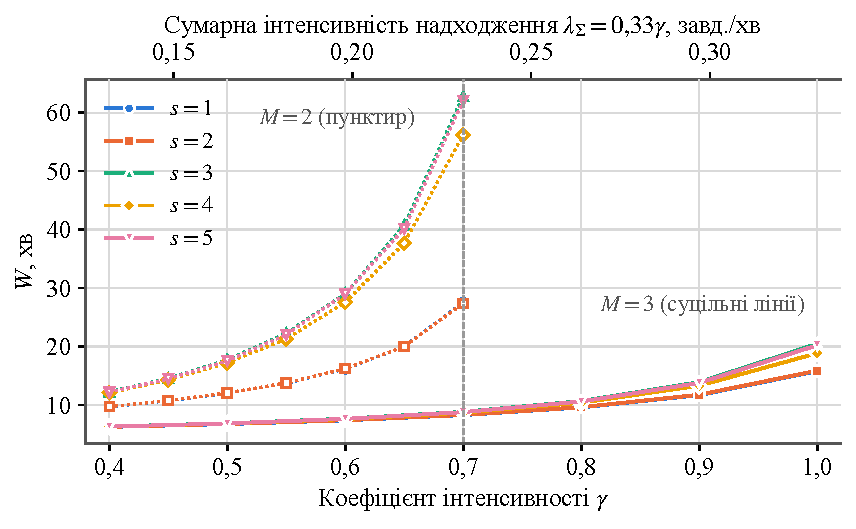
\includegraphics[width=0.7\textwidth]{media/imp-w}
  \caption{Середній час перебування в системі з памʼяттю $M = 2$ і $M = 3$
    ($T_{\text{мод}} = 3{,}5\cdot10^6$~хв, $T_{\text{п}} = 2\cdot10^4$~хв, 60~прогонів; штрихова
    вертикаль -- межа діапазону за $M = 2$)}
  \label{fig:imp-w}
\end{figure}

% Згенеровано experiments/analysis.py — не редагувати вручну
\begin{kpitable}{|c|r|r|r|r|r|r|r|}{Відгуки системи з памʼяттю $M = 3$ за інтенсивностей з умови задачі ($\gamma = 1$, 60 прогонів, $T_{\text{мод}} = 3{,}5\cdot10^6$~хв, $T_{\text{п}} = 2\cdot10^4$~хв)\label{tab:imp-base}}
  {\textbf{$s$} & \textbf{$W$, хв} & \textbf{$L_q$, завд.} & \textbf{$W_q$, хв} & \textbf{$W_A$, хв} & \textbf{$W_B$, хв} & \textbf{$W_C$, хв} & \textbf{$U$}}
  1 & 15,80 $\pm$ 0,04 & 3,46 $\pm$ 0,01 & 10,50 $\pm$ 0,04 & 6,4 & 9,3 & 54,9 & 0,783 \\ \hline
  2 & 15,89 $\pm$ 0,05 & 3,49 $\pm$ 0,02 & 10,58 $\pm$ 0,05 & 7,4 & 6,8 & 54,8 & 0,783 \\ \hline
  3 & 20,46 $\pm$ 0,06 & 5,00 $\pm$ 0,02 & 15,16 $\pm$ 0,06 & 22,9 & 8,3 & 26,5 & 0,784 \\ \hline
  4 & 18,87 $\pm$ 0,06 & 4,48 $\pm$ 0,02 & 13,57 $\pm$ 0,06 & 10,2 & 37,0 & 26,5 & 0,783 \\ \hline
  5 & 20,23 $\pm$ 0,06 & 4,93 $\pm$ 0,02 & 14,92 $\pm$ 0,06 & 21,2 & 12,2 & 26,5 & 0,783 \\ \hline
\end{kpitable}


% Згенеровано experiments/analysis.py — не редагувати вручну
\begin{kpitable}{|c|r|r|r|r|r|r|r|r|r|}{Порівняння відгуків за обсягу памʼяті $M = 2$ і $M = 3$ ($\gamma = 0{,}7$, 60 прогонів, $T_{\text{мод}} = 3{,}5\cdot10^6$~хв, $T_{\text{п}} = 2\cdot10^4$~хв)\label{tab:imp-compare}}
  { & \multicolumn{3}{c|}{\textbf{$W$, хв}} & \multicolumn{3}{c|}{\textbf{$L_q$, завд.}} & \multicolumn{3}{c|}{\textbf{$W_q$, хв}} \\ \cline{2-10}
  \textbf{$s$} & \textbf{$M = 2$} & \textbf{$M = 3$} & \textbf{$\Delta$, \%} & \textbf{$M = 2$} & \textbf{$M = 3$} & \textbf{$\Delta$, \%} & \textbf{$M = 2$} & \textbf{$M = 3$} & \textbf{$\Delta$, \%}}
  1 & 27,53 & 8,29 & $-$70 & 5,14 & 0,69 & $-$87 & 22,23 & 2,99 & $-$87 \\ \hline
  2 & 27,40 & 8,31 & $-$70 & 5,11 & 0,69 & $-$86 & 22,10 & 3,01 & $-$86 \\ \hline
  3 & 62,82 & 8,83 & $-$86 & 13,29 & 0,81 & $-$94 & 57,52 & 3,53 & $-$94 \\ \hline
  4 & 56,20 & 8,70 & $-$85 & 11,75 & 0,78 & $-$93 & 50,90 & 3,40 & $-$93 \\ \hline
  5 & 62,04 & 8,79 & $-$86 & 13,10 & 0,81 & $-$94 & 56,73 & 3,49 & $-$94 \\ \hline
\end{kpitable}


Погіршення відгуків порівняно з $M = 2$ не виявлено (за $\gamma \le 0{,}7$ коротше перебувають
завдання всіх типів). Ціна зміни -- памʼять більша на 50~\% (за $\gamma = 0{,}7$ використання
падає з 0,82 до 0,55) і відмова від монопольного виконання~C; за потоку з умови задачі найдовше
знову чекає тип із найнижчим пріоритетом -- завдання~C у стратегіях 1--2 ($W_{q,C} = 45$~хв
проти 16,5~хв у 3--5) і завдання~B у стратегії~4 ($W_{q,B} = 32$~хв). Висновки щодо вибору
стратегії зберігаються й для системи з $M = 3$: за потоку з умови задачі стратегії 1--2 дають
середній час перебування на 16--23~\% менший, ніж стратегії 3--5 (таблиця~\ref{tab:imp-base}). Дешевша альтернатива -- стратегія 1 або~2 без зміни ресурсу -- за $\gamma = 0{,}7$ скорочує час
перебування у 2,0--2,3~раза, але не дає стійкості за потоку з умови; памʼять -- ще в 3,3~раза. Отже, за потоку, близького до заданого ($\gamma > 0{,}75$), збільшення памʼяті доцільне: лише
воно з розглянутих змін забезпечує роботу системи, а зі стратегією 1 або~2 дає найменший
середній час перебування (15,8~хв). За меншого потоку достатньо вибрати стратегію 1 або~2.

\subsection{Висновки до розділу}

Упорядкування перерозподіляє очікування: стратегії 1 і~2 найкращі загалом, якщо потік не
перевищує трьох чвертей заданого, стратегія~4 -- для завдань~C. Памʼять у три одиниці робить
систему стійкою за потоку з умови задачі й доцільна для нього.
